\documentclass{acm_proc_article-sp}

\usepackage{listings}
\lstset{language=C}
\usepackage{program}

\begin{document}

\title{02211 \\ Advanced Computer Architecture}
\subtitle{Group 4 Project Report - Design of a MIPS like processor}

\numberofauthors{3}
\author{
% 1st. author
\alignauthor Andreas Borup Svendsen\\
       \affaddr{Department of Informatics and Mathematical Modeling}\\
       \email{s072623@student.dtu.dk}
% 2nd. author
\alignauthor Attila S\"{u}k\"{o}sd\\
       \affaddr{Department of Informatics and Mathematical Modeling}\\
       \email{s070600@student.dtu.dk}
% 3rd. author
\alignauthor Kasper Grue Understrup\\
       \affaddr{Department of Informatics and Mathematical Modeling}\\
       \email{s061887@student.dtu.dk}
}

\maketitle

\begin{abstract}
This project presents a working MIPS like processor and assembler. The processor has been implemented from scratch in VHDL, as a learning experience. We have implemented the standard functions of the MIPS processor with forwarding and presented a UART and VGA output for debugging. The UART outputs via a serial cable, where the VGA output works through memory mapped I/O. We have been using ModelSim for testing and debugging. The assembler can be used to program our processor.

To demonstrate the full capabilities of the processor, a simple pong style game was implemented.
\end{abstract}

\section{Introduction}
This project aims at implementing a MIPS like processor architecture on an FPGA. The MIPS architecture was chosen based on its simplicity and widespread use, which allows the incorporation of ready-made stuff (such as the gcc-compiler) along the way, and compare the results of tests with those of a MIPS simulator.

As special features, forwarding and memory mapped I/O (VGA output and keyboard input) have been implemented. A pong game has also been developed, in order to demonstrate the capabilities of our processor.

\begin{figure}[!h]
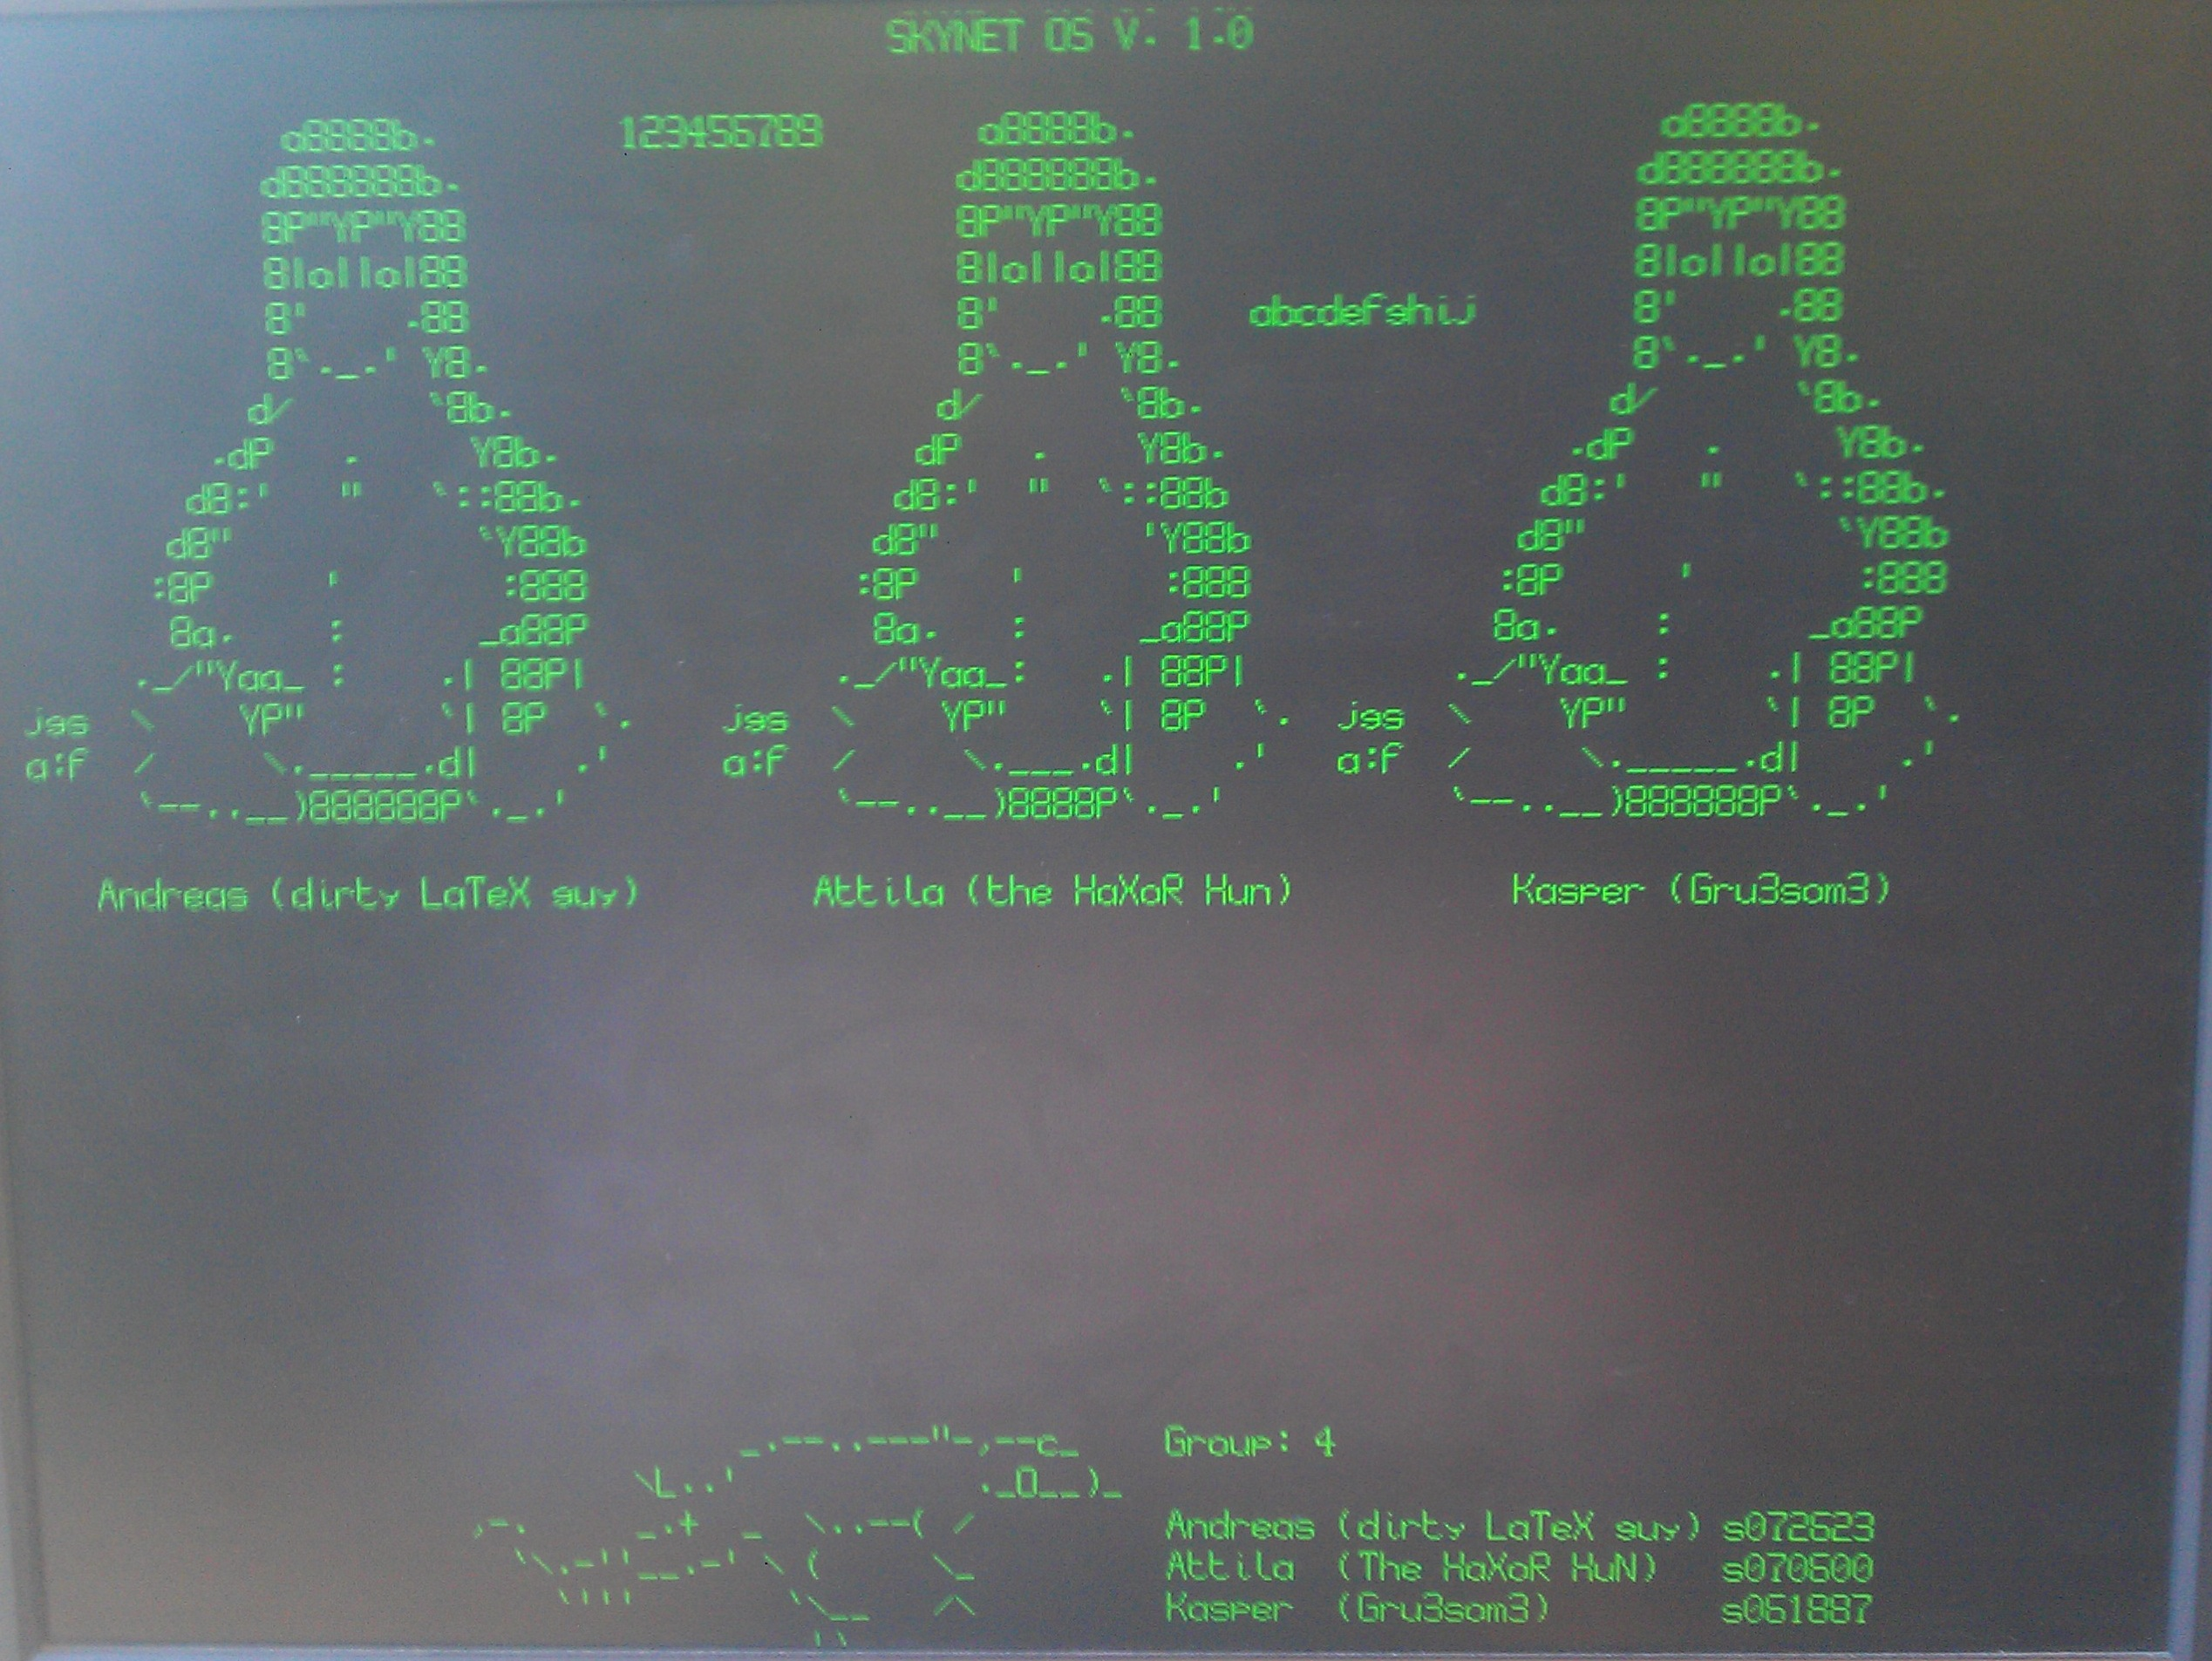
\includegraphics[width=0.45\textwidth]{Images/screen.jpg}
\caption{Splash screen for the pong game.}
\label{fig:splash}
\end{figure}

\paragraph{Outline} After this introductory section, a more thorough introduction to the MIPS architecture and the alternatives to the MIPS is given in section \ref{MIPS}. Section \ref{sec:implementation} deals with the design choices made, and the practical aspects of implementing our MIPS like processor. In section \ref{running} we describe how programs can be compiled and run, and in section \ref{testing} the tests performed are described, along with subsections describing troubles along the way, and relevant suggestions for further improvements in section \ref{sec:future}. Finally, conclusions are drawn in section \ref{conclusion}. The complete list of instructions implemented, along with some relevant code snippets are presented in the Appendix.

\subsection{The MIPS processor}
The MIPS (which is an acronym for Microprocessor without Interlocked Pipeline Stages) processor was first introduced in 1981 by the Company MIPS Technologies. The original MIPS processor was a 32-bit machine, however, newer versions are 64-bit, and it is based on a RISC instruction set architecture (ISA), which simplifies the hardware. The processor implemented in this project, is based on the original 32-bit MIPS.





\subsection{Motivation}
The MIPS instruction set is well tested, and has a lot of advantages. The fixed length 32-bit instruction words allow for smarter hardware implementation, especially since the structure of the instruction words is fixed, so that instructions can be passed on through pipelined stages and be decoded along the way, instead of having to be decoded all at once.

By using the almost\footnote{Due to time constraints, not all instructions of the MIPS core instruction set were implemented. These are the byte and halfword instructions along with the conditional store} full core instruction set (as seen in Appendix \ref{list}), we have the advantage of being able to compile real programs into MIPS assembler code, which can be run directly on our processor. Had we instead chosen to work on a modified version of the MIPS instruction set or a smaller subset, a compiler would have had to be written from scratch, or any program that was to run on the processor would have to be written in assembler. Both these solutions would involve a lot of work, which would not be directly relevant for the purpose of this course\footnote{As it turns out, some extra effort still had to be put into the code translation, since there were a few bugs in the gcc MIPS compiler as described in section \ref{sec:gcc}}. With the chosen subset of instructions, only small modifications had to be made to the assembler code generated by the gcc, before it could run.


\section{MIPS design}\label{MIPS}
The strength of the MIPS processor is its fixed and simple RISC instruction set and its simple and non overlapping pipeline stages. Three types of instructions exist in the set. R-types which is the registry format, I-type which is the immediate format and J-type which is the jump format. These instructions are 32-bit wide in a 32-bit machine and arranged as shown in Figure \ref{fig:ISA}. % Why the fuck does this reference go wrong???

\begin{figure}[!h] 
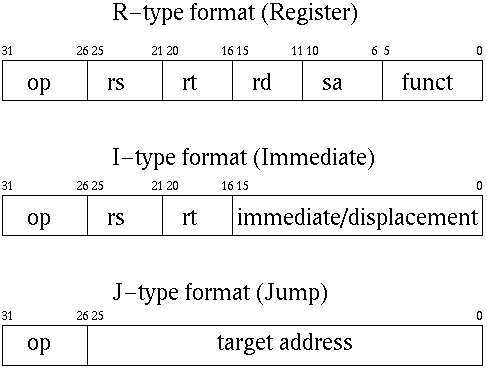
\includegraphics[width=0.45\textwidth]{Images/image.png}
\caption{MIPS instruction types}
\label{fig:ISA}
\end{figure}

In the following section, the theory behind the MIPS processor architecture, and some aspects of processors in general are introduced. Some things were implemented in our processor, while others (such as caching and branch prediction) were unfortunately left out due to time constraints. Most of the theory section is based on \cite{Patterson:2008:COD:1502247} and \cite{CompArch}.

\subsection{Processor Architecture}
In order to speed up modern processors, parallelism has to be exploited. One way to achieve this is through pipelining. By dividing instruction into sub instructions, a new instruction can be started right after the previous sub instruction has finished. The maximum speed up of pipelining is equal to the number of pipeline stages. However, pipelining introduces a number of problems due to dependencies. These problems can be categorized as structural hazards, data hazards and control hazards.

To deal effectively with these hazards, forwarding and branch prediction has to be introduced. Our processor is pipelined into five independent stages and therefore the maximum speed up of our processor compared to the non-pipeline alternative is 5. The five pipeline stages of the MIPS processor is: Instruction fetch, Instruction decode, Execute, Memory access and Write back.

Due to Moore's law, the size and price of semi conductors has decreased dramatically. This has spawned new processor designs which implement parallelism and pipelining. At the same time memory modules have not been evolving at the same pace, making memory one of the biggest bottlenecks in modern computers. Modern processors can process huge amount of data, but without efficient memory, these processors have to stall in order for the memory module to respond.

The ideal memory has a low response time and at the same time an unlimited amount of storage. This is extremely expensive because fast memory is expensive. however it is possible to create an illusion of a big fast memory by introducing memory hierarchy. Because slow memory is cheap, a large part of the memory should be build by slow memory, layers of faster and faster and smaller and smaller memory modules should be build on top of the slower memory modules. The processor should then communicate mostly with upper levels of the memory modules which would decrease latency of the module.

To take advantage of a memory hierarchy the memory should be build with spatial and temporal locality in mind. Spatial locality is a concept of loading data close to the fetched data in to upper level of the memory, whereas temporal locality is a concept of reusing data that has previously been used.

The caches of today which is the upper part of the memory hierarchy are located at the CPU chip. A big part of the CPU chip today is in fact cache in different levels. L1 and L2 caches are usually small memory units, which can only be accessed by one core, while L3 caches are bigger and can be accessed by multiple core depending on the architecture. An example of such a cache hierarchy can be seen in Figure \ref{cache}.

\begin{figure}[!h] 
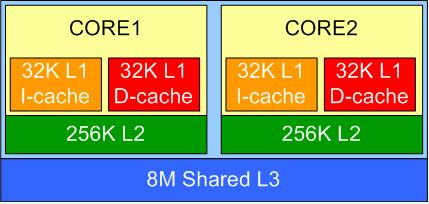
\includegraphics[width=0.45\textwidth]{Images/Cache_level.JPG}
\caption{On chip cache}
\label{cache}
\end{figure}


Main memory is located outside the CPU chip and is the slowest part of the memory hierarchy. A typical modern main memory in a desktop or laptop PC is around 4 to 8 Gb of storage. If there is a cache miss, and data has to be fetched from main memory, the penalty is in the range of thousands of clock cycles depending on the technology. 

In the eighties and nineties processors got more and more advanced, and computer designers only had to think about speed of the components. Pipeline stages and complexity exploded to get that extra speed, and thus the frequency in which the processor operated increased. When the computer designers hit the power wall, a whole new challenge was introduces: how to go fast without dissipating to much power. There is a fixed amount of power that can be dissipated without melting the chip. A processor that runs at 4 GHz but consumes more than double the power of a 2 GHz processor is actually quite often slower. This is because the of parallelism implemented in today's CPUs. The reason computer designers hit the power wall is because of the following equation:

\begin{eqnarray}
\label{Power Dissipation}
P = CV^2f 
\end{eqnarray}

This equation states that the power dissipation is equal to the capacitance times the voltage squared times the switching frequency. Since the voltage level and the capacitance are largely dependent on the CMOS technology used to produce the chip, these are normally outside the control of the hardware designer. However, by lowering the frequency and create more efficient pipeline stages, it is possible to reduce the power consumption without reducing the throughput. 

Because power dissipation is the limiting factor units can be shut down when they are not used. This can be done by removing the clock signal or the power to the unit. 

\subsection{Hazards}
There are three types of hazards to deal with as a computer designer: Structural hazards, data hazards and control hazards. Structural hazards occur when a combination of instructions is not supported by the architecture. This can happen if two functions at the same time try to use the ALU, or if a register is both written to and read from at the same time. In this case some data can be lost due to a structural hazard. Due to the fixed and independent pipeline structure of the MIPS processor, structural hazards should not occur. %?? unless only single register between pipeline stages is implemented. 

Data hazards occur when data from one instruction is to be used in one of the following instructions dependent of the instruction. The following example shows a data hazard:

\begin{itemize}
\item[] Add \$4, \$5, \$6 \# add1
\item[] Add \$3, \$4, \$5 \# add2
\end{itemize}

The value of register four is available after the fifth stage in the pipeline of the first add instruction. The register read of the second add instruction has however to be present in the second stage. If there is no hardware solution to the problem bubbles or NOP operations have to be inserted between the lines in the assembler code. NOP operations consist of all zeros\footnote{This translates into sll 0 \$0, \$0, \$0, which means that the contents of register zero should be left shifted by zero places and stored back. This, of course, does nothing to the data.}, and are inserted to instruct the processor to do nothing for one clock period. The hardware solution is to insert forwarding which allows the two add operations to be executed right after each other. The data is written back to the register in stage five, but with forwarding the second add instruction can read the the result of the first add operation directly, and thus does not have to wait for it to be stored in the register.

A data hazard, that cannot be solved by forwarding, is the hazard that occurs, when a value loaded from memory is to be used in the subsequent instruction. Since the data is not fetched from memory until the memory access (MEM) stage, and the data is to be used in the execute stage (EX) of the subsequent instruction, it is impossible to solve this dependency by forwarding.This means, that even with forwarding, at least one bubble (NOP) has to be inserted if the value of this function has to be used in the next. To optimize the performance the program can be optimized at assembler level to remove as many data hazards as possible, by rearranging the code. This is, however, more of a software problem than a hardware problem. This example shows that a computer designer both has to be aware of software and hardware implementations in order to be successful. In our design we have implemented forwarding and thus NOPs do not have to be inserted at every dependency. 

The last hazard is control hazards; these hazards occur when branching. The processor cannot know in advance whether to branch or not, and therefore NOPs have to be implemented after a branch. There are many approaches to branch prediction, and some of them can predict the result with great accuracy, but since we have not implemented branch prediction we will not discuss it further. In our design NOPs have to be inserted manually in the assembler after every LW and branch instructions. If a C program is compiled using the gcc compiler, this program has to be investigated in order to manually insert the necessary NOPs.



\subsection{Pipeline stages}

In order to build a pipeline, many things have to be taken into account. The slowest pipeline stage determines the maximum frequency at which the processor runs. The instructions have to be passed down the pipeline, and the decoding can be done as the instruction is being executed. The MIPS pipeline is divided into five non interlocked pipeline stages as shown in Figure \ref{pipelinestages}. Most of the wires in the picture are buses which means a bunch of wires which hold and transfer a given value or instruction.

\begin{figure}[!h]
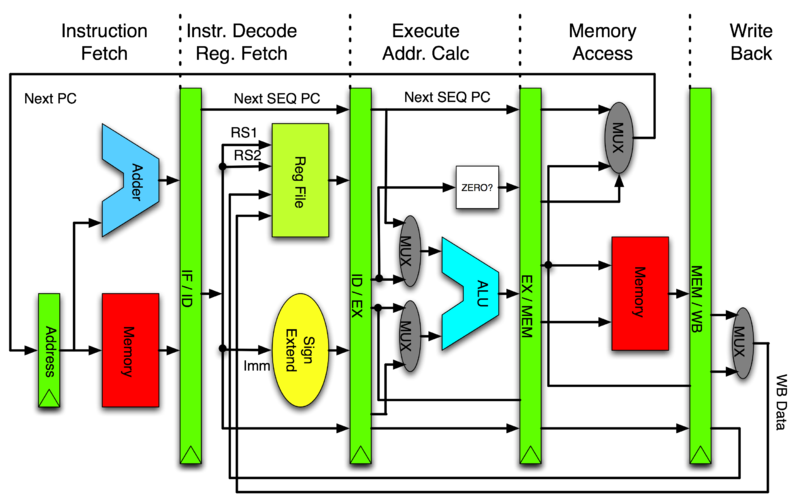
\includegraphics[width=0.45\textwidth]{Images/pipemips.png}
\caption{MIPS pipeline stages}
\label{pipelinestages}
\end{figure}

\subsubsection{IF: Instruction fetch}

In this stage the 32-bit instruction is being fetched from the memory using the address from the program counter. This instruction is stored in the IF/ID pipeline register. The address is then incremented by four since there are four bytes per word. The processor cannot at this stage know what type of instruction is fetched, so it must prepare for any instruction, and passing all potentially needed information to the next stage in the pipeline. 

A number of control signals are fed back to this stage from later stages, in order to handle jumps and branches, that require the program counter to be altered.

\subsubsection{ID: Instruction decode}

In this stage, the contents of two registers are fetched, based on the instruction word propagated from the IF/ID pipeline register. The two 32 bit values are then stored in the ID/EX registers. At this point the type of instruction is still not determined, so the registers are read, regardless of whether they are needed or not. Because this stage is executed regardless of the instruction no control signals are needed, but the control signals for the subsequent stages are extracted here, and propagated along in the pipeline registers.

\subsubsection{EX: Execute stage}

In this stage different things can happen,  on of the values of the read register is passed on to the EX/MEM pipeline register to be used in case of a memory operation. The two register values can be processed by an arithmetic operation in the ALU and passed on to the EX/MEM register. The instruction can be a branch or a jump instruction and thus a new PC can be calculated. The value of the new PC is stored in the EX/MEM pipeline registers.

In this stage, a number of control signals are needed. The control signal for this stage contains three values that control different multiplexers: an ALU control, a register control and a PC control. The MUX for the PC is not directly controlled, but the signal value is stored in the EX/MEM pipeline register.  

\subsubsection{MEM: Memory stage}

The MEM stage reads the EX/MEM pipeline registers and reads from, or writes to the main memory. In case of a read, the data is passed to the MEM/WB pipeline register. This is the stage where the jump functions take effect and the PC is updated. The thing to notice is jump functions only take four stages in the MIPS pipeline compared to all other functions that takes five. If the jump function is a reality the pipeline, given that the branch prediction was wrong, has to be flushed. Two control signals are needed in this stage, one to control the memory read or write and the second is for branching.

\subsubsection{WB: Write back}

The write back stage reads the MEM/WB pipeline register and stores the value back into the registers. If the instruction was a memory write, a jump function or a NOP nothing happens in this stage. This stage is the final stage in the MIPS pipeline, and thus the instruction is completed after this step. Some of the more advanced arithmetic operations (multiply, divide etc.) are exceptions to this rule, as they take multiple clock cycles to complete. However, they are performed in the backgroung, and the result will be written to reserved registers, when they are ready. It is therefore up to the compiler / programmer, to make sure that the data is ready, before attempting to read the result. If this \textit{background} approach is not taken, the frequency of the processor has to be lowered to fit the complex instructions, which would severely increase the latency and thus lower the throughput of the processor. 



\subsection{Other approaches}
Before settling on the MIPS architecture, a number of other RISC instruction sets were considered. These are briefly described in the following section.

\subsubsection{The ARM architecture}
ARM (Advanced RISC Machine) is a 32-bit reduced instruction set computer (RISC) instruction set architecture (ISA). ARM has evolved over time, with the most recent revision defining three profiles: application, real-time and microcontroller. Each profile adds various instructions, so, in order to keep it simple, the following will consider the original implementation of ARM. Originally ARM was hardwired without microcode in order to keep the design clean. It included the following RISC features:

\begin{itemize}
\item Load/store architecture.
\item No support for misaligned memory accesses.
\item Uniform 32-bit register file.
\item Fixed instruction width of 32 bits.
\item Mostly single-cycle execution.
\end{itemize}

Some additional design features were used to compensate for the simple design:

\begin{itemize}
\item Conditional execution of most instructions, in order to reduce branch overhead and compensate for the lack of a branch predictor.
\item Arithmetic instructions only alter condition codes when desired.
\item 32-bit barrel shifter which can be used without performance penalty with most arithmetic instructions and address calculations.
\item Powerful indexed addressing modes.
\item A link register for fast leaf function calls.
\item Simple, but fast, 2-priority-level interrupt subsystem with switched register banks.
\end{itemize}
Newer revisions now have support for misaligned memory accesses, with some exceptions related to load/store multiple word instructions. ARM has 37 Registers in total, all of which are 32-bits long. These are used as follows:
\begin{itemize}
\item 1 dedicated program counter
\item 1 dedicated current program status register
\item 5 dedicated saved program status registers
\item 30 general purpose registers
\end{itemize}
Earlier ARM implementations have a three stage pipeline, the stages being: fetch, decode and execute. Later designs have deeper pipelines for higher performance. The ARM processor used in iPhone 3GS has 13 stages. Other features and instructions have been developed to enhance performance, particularly the applications profile has been enhanced for multimedia performance.







\subsubsection{The PIC architecture}
With over 10 billion PIC microcontrollers sold world-wide as of September 2011\footnote{http://www.microchip.com/pagehandler/en-us/press-release/microchip-technology-delivers-10-billionth-pic-mic.html}, the RISC based PIC family is one the most common architectures around. The instruction set has been expanded over the years, but in the following, we have chosen to focus on the PIC16 instruction set with just 35 instructions (even though an even simpler 12-bit instruction word set with 32 instructions exists).

The instruction set is of the accumulator type, which means that many instructions use an implied accumulator register called W0, which allows for shorter opcodes, since the register address is not needed in the instruction. These instructions often have a 1-bit input operand called d, which allows selecting whether to write the result to the accumulator register or to the other register involved.
The instructions are 14-bit words, and can be divided into four general categories:
\begin{itemize}
\item Byte-oriented file register operations
\begin{itemize}
\item Operations on byte values, in the accumulator register and one additional register.
\end{itemize}
\item Bit-oriented file register operations
\begin{itemize}
\item Operations that test and/or set specific bits in a register.
\end{itemize}
\item Literal operations
\begin{itemize}
\item Operations on the accumulator register with a byte value given as the 8 LSB of the instruction
\end{itemize}
\item Control operations
\begin{itemize}
\item Sleep, Goto, Return etc.
\end{itemize}
\end{itemize}
The instruction set supports 128 8-bit registers, of which the first 32 are reserved for special purpose registers, and the remaining 96 bytes are available as regular RAM.



\section{Design and implementation} \label{sec:implementation}
The MIPS like processor has been implemented in VHDL from scratch. The overall structure of the design is described below.

\subsection{The MIPS like design}

The top level component in our design is the \texttt{MIPSlike.vhd}; this file links each pipeline stage together. For simplicity we have been using the divide and conquer strategy and split the functionalities into several files. We have a separate file for each pipeline stage, the memory some MUXes and a ROM for our program. This helps debugging the code since units can be tested separately.

The Instruction fetch stage is located in the \texttt{instructionFetch.vhd} file. This stage takes care of updating the program counter, and fetches the instruction from the program ROM. It takes some control signals for branching and jumping as inputs, and outputs a 32-bit instruction and a 32-bit program counter.

The Instruction decode is located in the \texttt{instructionDecode.vhd} file. This stage reads the opcode of the instruction, which is the first six bits of the instruction. In our MIPS like processor, we have implemented all the basic functionalities of the MIPS architecture. We have, however, not implemented all the functionalities of the RISC architecture, we have not implemented a floating point unit and therefore floating point operations are not part of our MIPS like processor. For a detailed list of the supported functions view Appendix \ref{list}. There are many outputs from this stage since this stage determines what the processor must do.

A potential problem that can come up in the IF stage is where the same register is being written to, while it is being read from. In many MIPS implementations, this is avoided by using opposite clock polarity, when doing reads and writes \footnote{E.g. writing on the rising edge of the clock and reading on the falling edge}. In our processor, a slightly different approach has been taken, and the registers being read and written are simply compared, and in case of a match, the data being written is forwarded to the output.

The execute stage is split into two, where the forwarding logic is implemented in the \texttt{Forwarding.vhd} component, and the arithmetic parts are implemented in the \texttt{Execute.vhd} file.

The forwarding stage compares the contents of the different pipeline registers with the data being processed, and replaces the data read from the register with a more recent version of the data, if one such exists. This way, some data hazards can be resolved without the need for stalling the processor.

The execute stage contains the ALU, which is the arithmetic logic unit of the processor. We have implemented the basic functionality of the MIPS ISA, but some complex functions have been left out of the current version. For instance, a modern processor should also be able to deal with floating point formats which has a magnitude, an exponent and a sign extension. This format increases the range of numbers but also needs specific hardware, and as such has not been implemented. So this would probably have to be implemented before we attempt to sell our design.

The memory access stage is located in the \texttt{memoryAccess.vhd} file. In this stage the memory can be accessed, by either reading from the memory or writing to it. % We have chosen to use a dual-port ram since it makes it possible to have two memory accesses at the same time.

The Write back stage is located in the \texttt{WriteBack.vhd} file. In this stage the result of the ALU or the memory is written back to the registry if needed.

Furthermore, keyboard input and VGA output have been implemented using memory mapped I/O.
% Something about memory addresses and such??

\subsection{FPGAimplementation}
Our MIPS processor is implemented on the Spartan 3E-1600 Development Board\footnote{http://www.digilent.ro/Products/Detail.cfm?NavPath=\\2,400,793\&Prod=S3E1600} as shown in Figure \ref{fig:fpga}. This board has 1.6 M gates, a serial output and a 50 MHz clock. The board is somewhat different from the Altera Cyclone FPGA in the hardware lab. The Spartan board has fewer input buttons but has significantly more logic units, allowing for bigger designs. The Development environment is also different; to program the Spartan board, the Xilinx ISE design suite and Impact is the only choice, whereas the Quartus software must be used to design hardware for the Altera board. These environments are, of course, different to use.

\begin{figure}[!h]
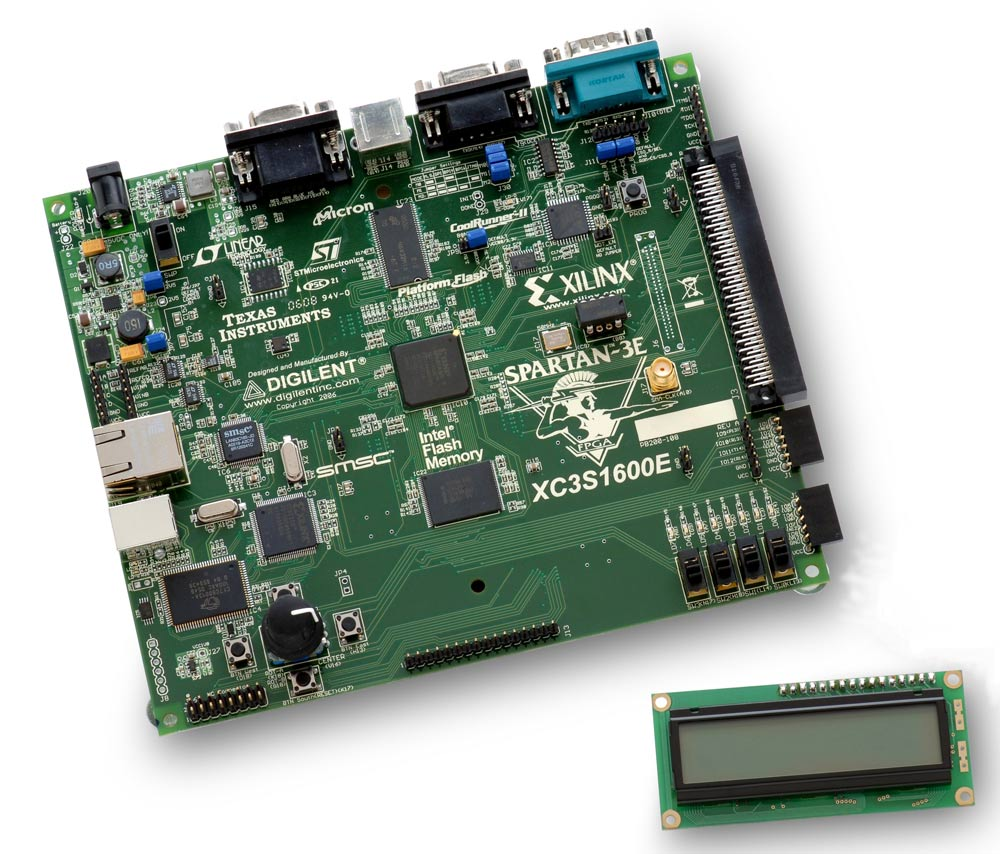
\includegraphics[width=0.45\textwidth]{Images/Xilinx.jpg}
\caption{Spartan 3E-1600 Development Board}
\label{fig:fpga}
\end{figure}

\section{Running code on the MIPS like design}\label{running}

The system calls from a typical C-program like \texttt{printf()} can of course not be implemented without an operating system, but the printf() can be outputted via the UART. 

The assembler is located in the \texttt{assembler.c} file. This file takes a program file as input and delivers an output file named \texttt{outputFile} with no extension. To use the assembler, the c program must be compiled and run like this: \texttt{./assembler} ''program''. The Assembler implements out commenting, easy extension for new instructions, string handling and register renaming. % The assembler could assembles this code:

To run these instructions on the MIPS, we have created a python program (\texttt{rommaker.py}) that inserts the machine code into a VHDL template. The template is called \texttt{rom.vhd} and is located in the ''MIPSlike'' folder. Ideally the instructions would load into an instruction cache but in our processor we hardcode it in the logic cells of the FPGA. We constructed a simple C program that calculates the Fibonacci Series. The program is shown in the appendix section \ref{C Code}. This code can be compiled into assembler code by applying the gcc compiler with the -S option, like this:
\begin{itemize}
\item[]gcc -S fibonacci.c
\end{itemize}
The obtained assembler code is shown in section \ref{assembler} with our comments. This code can then using our compiler be turned into machine code that works on our MIPS like processor. The command to do this is:

\begin{itemize}
\item[]./assembler "fibonacci.S"
\end{itemize}

\section{Test}\label{testing}
To test the processor we did several things. First we did a reverse string test, then a Fibbonaci program and lastly a Pong game. The reverse string and the Fibbonaci programs were outputted via the serial. The Pong game had input from a computer keyboard via a serial cable to control the flipper, a ball that was flying around with edge detection and VGA output to show the game on a computer screen. 

\begin{figure}[!h]
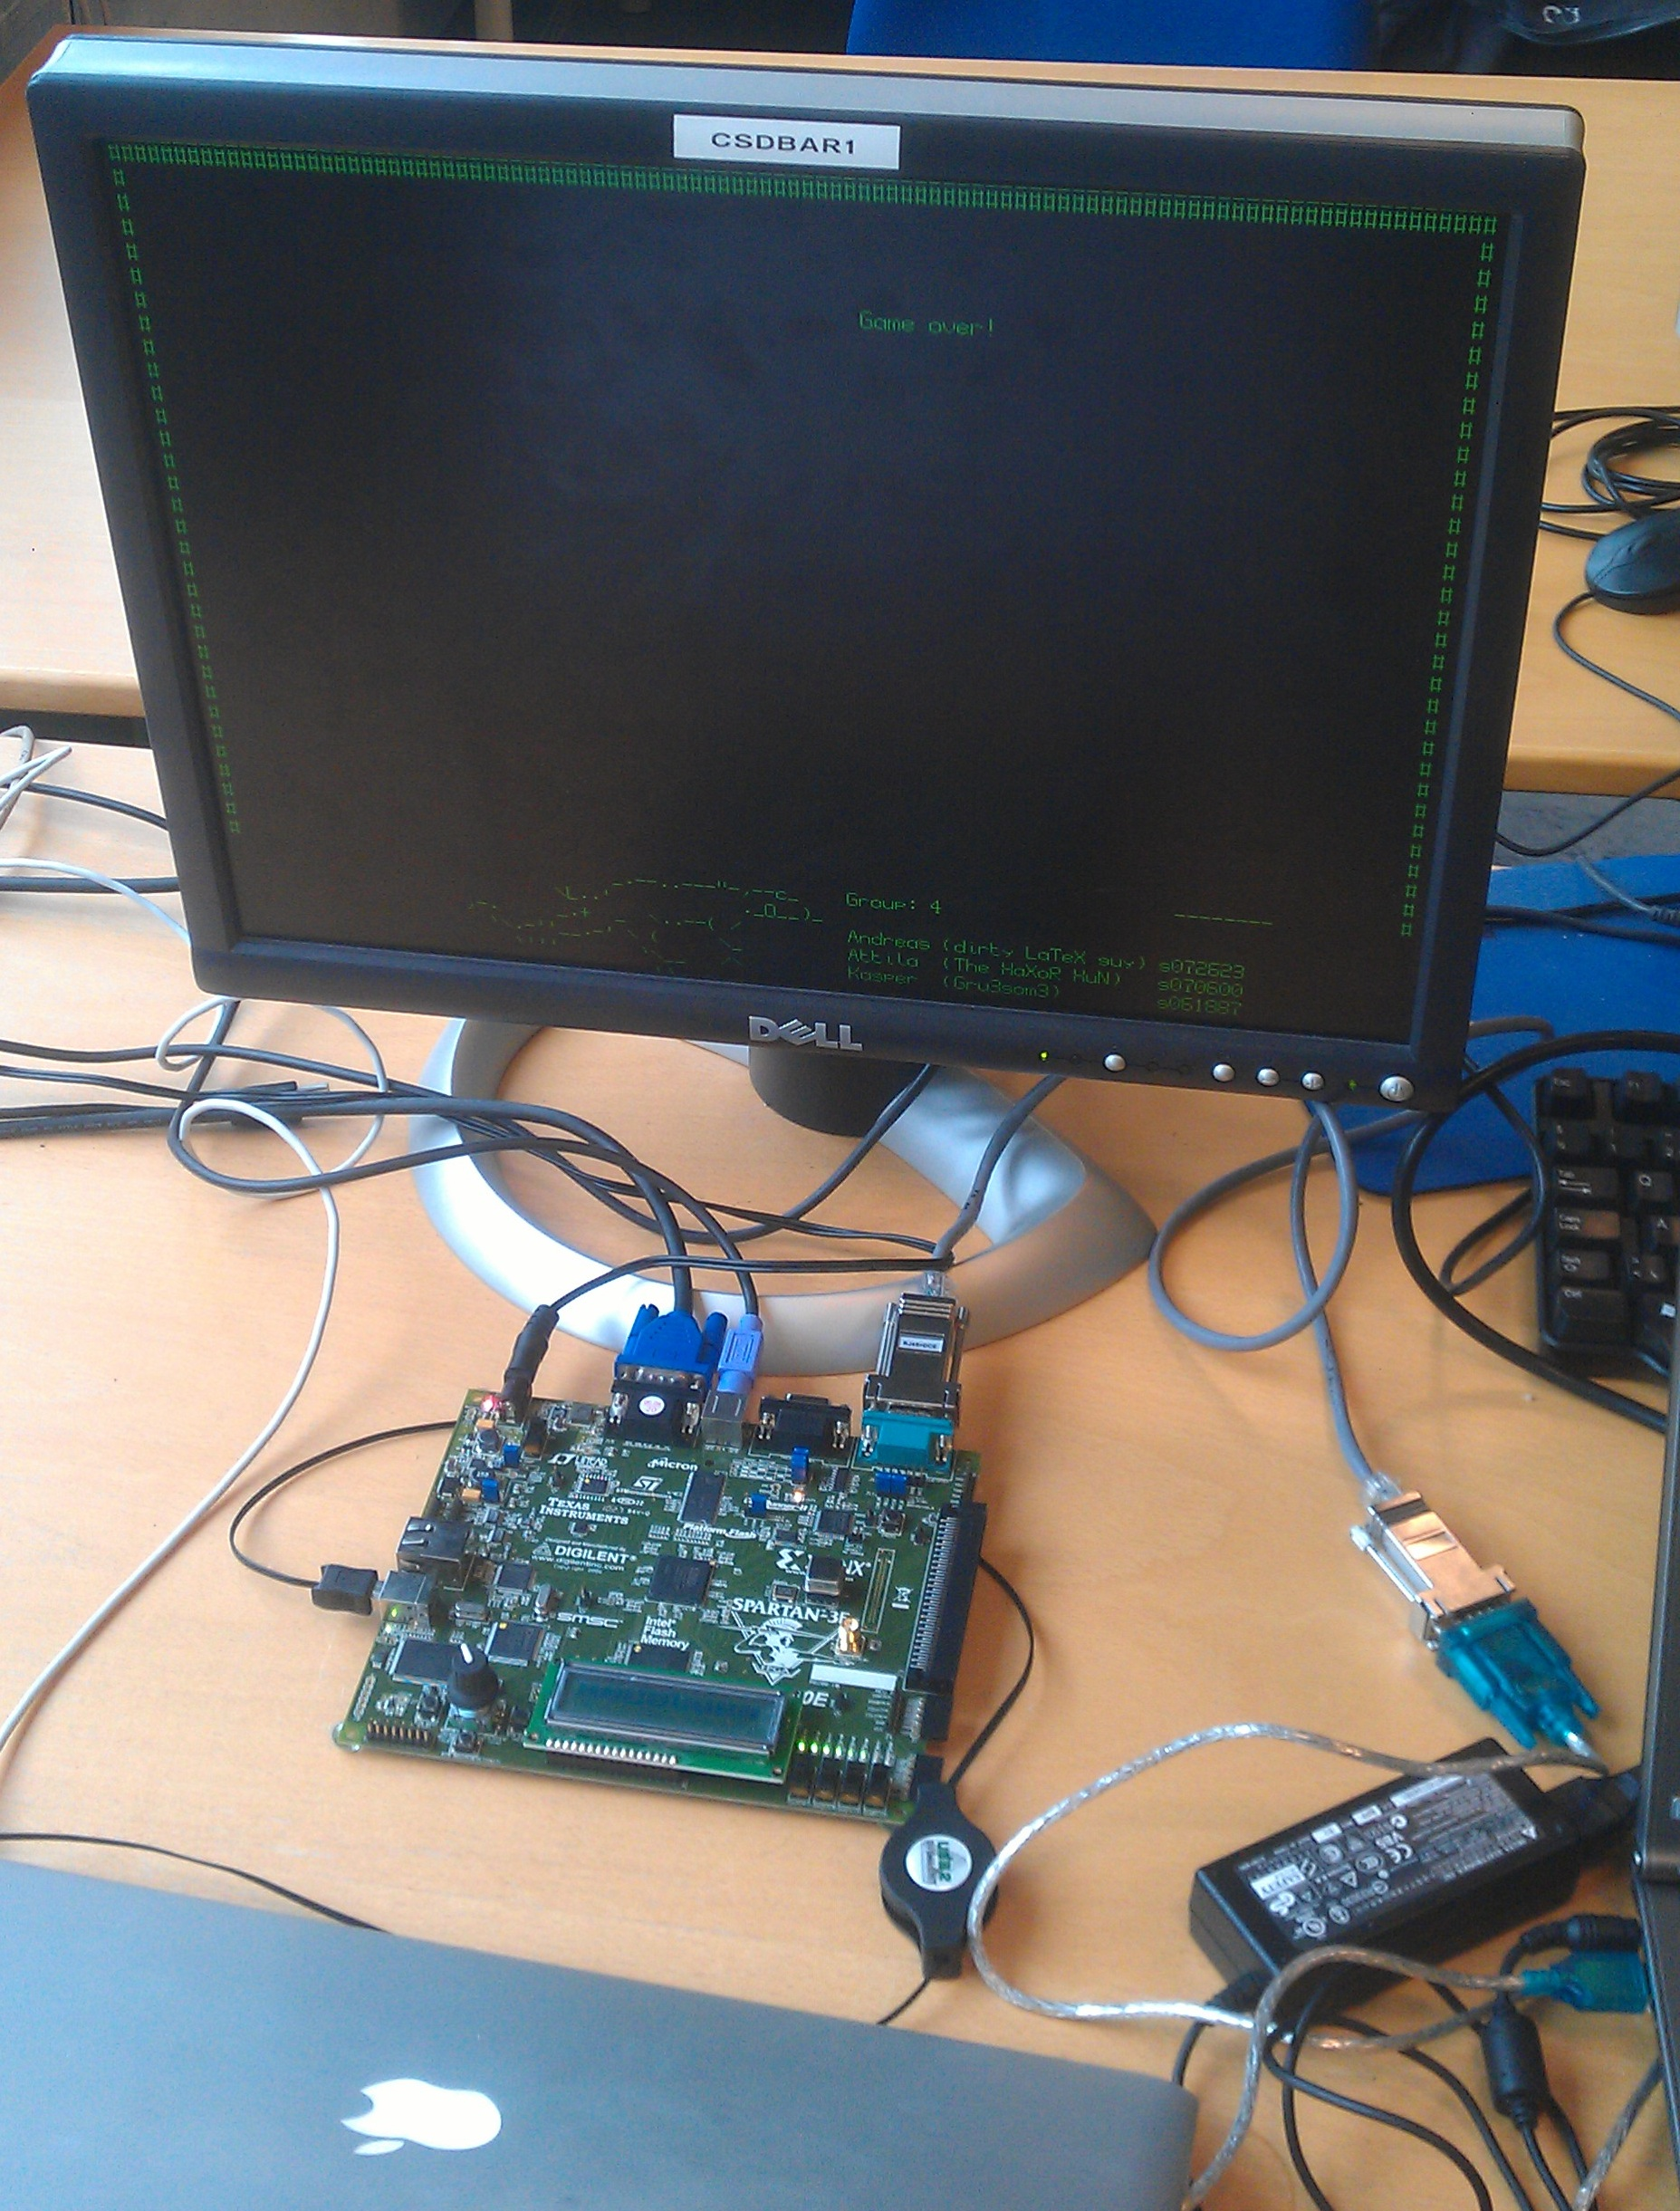
\includegraphics[width=0.45\textwidth]{Images/pong.jpg}
\caption{The pong game running on the MIPS on the FPGA.}
\label{fig:pong}
\end{figure}

As the programs grew in complexity our processor still managed to run them. In the Pong game we reached over a thousand lines of assembler code. Since we didn't implement all the functionalities in the MIPS processor, we sometime had to manually change some MIPS instructions to get the C program to work. However, with the implemented instructions, all MIPS core instructions could be emulated as pseudo instructions.


\subsection{Fibonacci}
The program calculates the Fibonacci numbers. The Fibonacci numbers which can be observed in nature, and can be mathematically derived by formula \ref{fibo} or by using the program on our MIPS like processor.
\begin{eqnarray}\label{fibo}
F_n=F_{n-1}+F_{n-2}
\end{eqnarray}
The processor correctly outputs the following numbers: % as shown in figure ******
\begin{itemize}
\item[] 1, 1, 2, 3, 5, 8, 13, 21, 34, 55, 89, 144, \ldots
\end{itemize}

\subsection{GCC troubles} \label{sec:gcc}
Although originally one of the main reasons for going with the MIPS architecture, was the availability of ready-made compilers and simulators. However, through testing and developing, it has become clear that the MIPS package of the gcc-compiler is not working optimally. For instance, the gcc compiler occasionally outputs a line like

\begin{itemize}
\item[]  slt \$t1, \$t2, 10
\end{itemize}

which does not make sense in the MIPS code used in \cite{Patterson:2008:COD:1502247}, since it is a mixture of an R-type and an I-type instruction. These instructions have to be manually replaced with the \texttt{slti} instruction, so it matches the data provided.

Another issue with the compiler is, that it does not utilize the full range of registers. This does not produce wrong results, but it hurts performance, since the same value has to be loaded numerous times. This can also be fixed by manually renaming the relevant registers. However, this is a lot of work to keep track of, even for smaller programs.


\subsection{Future work} \label{sec:future}

A functioning MIPS processor is up and running, but we have not implemented all functions included in the MIPS instruction set. We hope to be able to expand the processors instruction set, and are currently considering a number of options. One obvious expansion could be the inclusion of floating point instructions, which would, of course, require an implementation of a floating point co-processor. This has the added advantage, that we would still be able to use existing compilers to generate our assembler code.

An alternative could be to expand the instruction set with new instructions (e.g. more elaborate one-cycle branch instructions such as 'branch if less than' or others). These would however require some sort of custom assembler code to be generated, but we will cross that bridge when (and if) we get to it. 

We could also implement hardware accelerators to do specific task like graphic accelerator or to calculate cash flows for economic systems. 

Finally, the memory structure and hierarchy could be organized and developed further. This could include using a bootloader to load programs into the onboard ROM on the FPGA, or implementing a cache structure.


\section{Conclusions}\label{conclusion}

We have implemented a basic working MIPS processor. The processor implements the basic functions allowing simple integer based programs to be compiled and run. Forwarding has been implemented to improve the performance of the processor, and simple I/O memory mapping provides an improved user experience.

The capabilities of the processor can be demonstrated by running a simple pong game, which not only showcases the memory mapped I/O, but also demonstrates the processor stability, and that the partial MIPS instruction set is sufficient to run even somewhat advanced programs consisting of more than a thousand instruction.

\bibliographystyle{abbrv}
\bibliography{report} 


\newpage

\appendix

\section{Implemented Functions} \label{list}

\begin{itemize}
\item ADD -- Add (with overflow)
\item ADDI -- Add immediate (with overflow)
\item ADDIU -- Add immediate unsigned (no overflow)
\item ADDU -- Add unsigned (no overflow)
\item AND -- Bitwise and
\item ANDI -- Bitwise and immediate
\item BEQ -- Branch on equal
%\item BGEZ -- Branch on greater than or equal to zero
%\item BGEZAL -- Branch on greater than or equal to zero and link
%\item BGTZ -- Branch on greater than zero
%\item BGTZ -- Branch on greater than zero
%\item BLTZ -- Branch on less than zero
%\item BLTZAL -- Branch on less than zero and link
\item BNE -- Branch on not equal
%\item DIV -- Divide
%\item DIVU -- Divide unsigned
\item J -- Jump
\item JAL -- Jump and link
\item JR -- Jump register
%\item LB -- Load byte
%\item LUI -- Load upper immediate
\item LW -- Load word
%\item MFHI -- Move from HI
%\item MFLO -- Move from LO
%\item MULT -- Multiply 
%\item MULTU -- Multiply unsigned
\item NOP -- no operation (Pseudo instruction)
\item NOR -- Bitwise not OR
\item OR -- Bitwise or
\item ORI -- Bitwise or immediate
%\item SB -- Store byte
\item SLL -- Shift left logical 
%\item SLLV -- Shift left logical variable
\item SLT -- Set on less than (signed)
\item SLTI -- Set on less than immediate (signed)
\item SLTIU -- Set on less than immediate unsigned
\item SLTU -- Set on less than unsigned
%\item SRA -- Shift right arithmetic
\item SRL -- Shift right logical
%\item SRLV -- Shift right logical variable
\item SUB -- Subtract
\item SUBU -- Subtract unsigned
\item SW -- Store word
%\item SYSCALL -- System call
\item XOR -- Bitwise exclusive or
\item XORI -- Bitwise exclusive or immediate

\end{itemize}
\newpage
\section{Fibbonacci C Code} \label{C Code}
The Fibonacci C code is listed below. The pong code is a bit too large to include in the report, but will be uploaded along with the digital handin.

\begin{lstlisting}
#include "standard.h"

int main ()
{
  int a = 0,f=5;
  while (1) {
	a = get_chr();
  	fibonacci(f);
	f++;
  }
  return 0;
}

int fibonacci(int n)
{
  int a = 0;
  int b = 1;
  int sum;
  int i;
  for (i=0;i<n;i++)
  {
    put_hex(a);
    put_chr(' ');
    sum = a + b;
    a = b;
    b = sum;
  }
  put_chr('\r');
  put_chr('\n');
  return 0;
}

\end{lstlisting}
\newpage
\section{Fibonacci Assembler code} \label{assembler}
\lstset{language={[x86masm]Assembler}}
\begin{lstlisting}
	.file	1 "fib.c"
	.section .mdebug.abi32
	.previous
	.abicalls
	.text
	.align	2
	.globl	put_chr
	.ent	put_chr
	.type	put_chr, @function
put_chr:
	.frame	$sp,24,$31
	.mask	0x00000000,0
	.fmask	0x00000000,0
	.set	noreorder
	.cpload	$25
	.set	reorder
	addiu	$sp,$sp,-24
	sw	$4,24($sp)
	sw	$0,8($sp)
	li	$2,16384
	sw	$2,12($sp)
	li	$2,49152
	sw	$2,16($sp)
$L2:
	lw	$2,8($sp)
	bne	$2,$0,$L3
	lw	$2,12($sp)
	lw	$2,0($2)
	andi	$2,$2,0x1
	sw	$2,8($sp)
	b	$L2
$L3:
	lw	$3,16($sp)
	lw	$2,24($sp)
	sw	$2,0($3)
	addiu	$sp,$sp,24
	j	$31
	.end	put_chr
	.align	2
	.globl	get_chr
	.ent	get_chr
	.type	get_chr, @function
get_chr:
	.frame	$sp,24,$31
	.mask	0x00000000,0
	.fmask	0x00000000,0
	.set	noreorder
	.cpload	$25
	.set	reorder
	addiu	$sp,$sp,-24
	sw	$0,8($sp)
	li	$2,16384
	sw	$2,12($sp)
	li	$2,49152
	sw	$2,16($sp)
$L5:
	lw	$2,8($sp)
	bne	$2,$0,$L6
	lw	$2,12($sp)
	lw	$2,0($2)
	andi	$2,$2,0x2
	sw	$2,8($sp)
	b	$L5
$L6:
	lw	$2,16($sp)
	lw	$2,0($2)
	addiu	$sp,$sp,24
	j	$31
	.end	get_chr
	.align	2
	.globl	_put_hex
	.ent	_put_hex
	.type	_put_hex, @function
_put_hex:
	.frame	$sp,32,$31
	.mask	0x80000000,-8
	.fmask	0x00000000,0
	.set	noreorder
	.cpload	$25
	.set	reorder
	addiu	$sp,$sp,-32
	sw	$31,24($sp)
	.cprestore	16
	sw	$4,32($sp)
	lw	$2,32($sp)
	slt	$2,$2,10
	bne	$2,$0,$L8
	lw	$2,32($sp)
	addiu	$2,$2,55
	move	$4,$2
	jal	put_chr
	b	$L7
$L8:
	lw	$2,32($sp)
	addiu	$2,$2,48
	move	$4,$2
	jal	put_chr
$L7:
	lw	$31,24($sp)
	addiu	$sp,$sp,32
	j	$31
	.end	_put_hex
	.align	2
	.globl	put_hex
	.ent	put_hex
	.type	put_hex, @function
put_hex:
	.frame	$sp,40,$31
	.mask	0x80000000,-8
	.fmask	0x00000000,0
	.set	noreorder
	.cpload	$25
	.set	reorder
	addiu	$sp,$sp,-40
	sw	$31,32($sp)
	.cprestore	16
	sw	$4,40($sp)
	lw	$2,40($sp)
	sw	$2,24($sp)
	lw	$2,24($sp)
	bne	$2,$0,$L12
	lw	$4,40($sp)
	jal	_put_hex
	b	$L10
$L12:
	lw	$2,24($sp)
	beq	$2,$0,$L10
	lw	$2,24($sp)
	andi	$2,$2,0xf
	sw	$2,28($sp)
	lw	$4,28($sp)
	jal	_put_hex
	lw	$2,24($sp)
	sra	$2,$2,4
	sw	$2,24($sp)
	b	$L12
$L10:
	lw	$31,32($sp)
	addiu	$sp,$sp,40
	j	$31
	.end	put_hex
	.align	2
	.globl	main
	.ent	main
	.type	main, @function
main:
	.frame	$sp,40,$31
	.mask	0x80000000,-8
	.fmask	0x00000000,0
	.set	noreorder
	.cpload	$25
	.set	reorder
	addiu	$sp,$sp,-40
	sw	$31,32($sp)
	.cprestore	16
	sw	$0,24($sp)
	li	$2,5
	sw	$2,28($sp)
$L15:
	jal	get_chr
	sw	$2,24($sp)
	lw	$4,28($sp)
	jal	fibonacci
	lw	$2,28($sp)
	addiu	$2,$2,1
	sw	$2,28($sp)
	b	$L15
	.end	main
	.align	2
	.globl	fibonacci
	.ent	fibonacci
	.type	fibonacci, @function
fibonacci:
	.frame	$sp,48,$31
	.mask	0x80000000,-8
	.fmask	0x00000000,0
	.set	noreorder
	.cpload	$25
	.set	reorder
	addiu	$sp,$sp,-48
	sw	$31,40($sp)
	.cprestore	16
	sw	$4,48($sp)
	sw	$0,24($sp)
	li	$2,1
	sw	$2,28($sp)
	sw	$0,36($sp)
$L18:
	lw	$2,36($sp)
	lw	$3,48($sp)
	slt	$2,$2,$3
	beq	$2,$0,$L19
	lw	$4,24($sp)
	jal	put_hex
	li	$4,32
	jal	put_chr
	lw	$3,24($sp)
	lw	$2,28($sp)
	addu	$2,$3,$2
	sw	$2,32($sp)
	lw	$2,28($sp)
	sw	$2,24($sp)
	lw	$2,32($sp)
	sw	$2,28($sp)
	lw	$2,36($sp)
	addiu	$2,$2,1
	sw	$2,36($sp)
	b	$L18
$L19:
	li	$4,13
	jal	put_chr
	li	$4,10
	jal	put_chr
	move	$2,$0
	lw	$31,40($sp)
	addiu	$sp,$sp,48
	j	$31
	.end	fibonacci
	.ident	"GCC: (GNU) 3.4.6"
\end{lstlisting}


% \section{Machine Code}\label{Machinecode}
% \begin{itemize}
\item[] 00100000000111010000001111111111
\item[] 00000000000000000000000000000000
\item[] 00001100000000000000000010111110
\item[] 00000000000000000000000000000000
\item[] 00000000000000000000000000000000
\item[] 00000000000000000000000000000000
\item[] 00000000000000000000000000000000
\item[] 00000000000000000000000000000000
\item[] 00000000000000000000000000000000
\item[] 00000000000000000000000000000000
\item[] 00001000000000000000000000000110
\item[] 00000000000000000000000000000000
\item[] 00000000000000000000000000000000
\item[] 00000000000000000000000000000000
\item[] 00100011101111011111111111101000
\item[] 10101111101001000000000000011000
\item[] 10101111101000000000000000001000
\item[] 00100000000000100010000000000000
\item[] 10101111101000100000000000001100
\item[] 00100000000000100010000000000001
\item[] 10101111101000100000000000010000
\item[] 10001111101000100000000000001000
\item[] 00000000000000000000000000000000
\item[] 00010100010000000000000000001101
\item[] 00000000000000000000000000000000
\item[] 00000000000000000000000000000000
\item[] 00000000000000000000000000000000
\item[] 10001111101000100000000000001100
\item[] 00000000000000000000000000000000
\item[] 10001100010000100000000000000000
\item[] 00000000000000000000000000000000
\item[] 00110000010000100000000000000001
\item[] 10101111101000100000000000001000
\item[] 00010000000000001111111111110011
\item[] 00000000000000000000000000000000
\item[] 00000000000000000000000000000000
\item[] 00000000000000000000000000000000
\item[] 10001111101000110000000000010000
\item[] 00000000000000000000000000000000
\item[] 10001111101000100000000000011000
\item[] 00000000000000000000000000000000
\item[] 10101100011000100000000000000000
\item[] 00100011101111010000000000011000
\item[] 00000011111000000000000000001000
\item[] 00000000000000000000000000000000
\item[] 00000000000000000000000000000000
\item[] 00000000000000000000000000000000
\item[] 00100011101111011111111111101000
\item[] 10101111101000000000000000001000
\item[] 00100000000000100010000000000000
\item[] 10101111101000100000000000001100
\item[] 00100000000000100010000000000001
\item[] 10101111101000100000000000010000
\item[] 10001111101000100000000000001000
\item[] 00000000000000000000000000000000
\item[] 00010100010000000000000000001101
\item[] 00000000000000000000000000000000
\item[] 00000000000000000000000000000000
\item[] 00000000000000000000000000000000
\item[] 10001111101000100000000000001100
\item[] 00000000000000000000000000000000
\item[] 10001100010000100000000000000000
\item[] 00000000000000000000000000000000
\item[] 00110000010000100000000000000010
\item[] 10101111101000100000000000001000
\item[] 00010000000000001111111111110011
\item[] 00000000000000000000000000000000
\item[] 00000000000000000000000000000000
\item[] 00000000000000000000000000000000
\item[] 10001111101000100000000000010000
\item[] 00000000000000000000000000000000
\item[] 10001100010000100000000000000000
\item[] 00000000000000000000000000000000
\item[] 00100011101111010000000000011000
\item[] 00000011111000000000000000001000
\item[] 00000000000000000000000000000000
\item[] 00000000000000000000000000000000
\item[] 00000000000000000000000000000000
\item[] 00100011101111011111111111100000
\item[] 10101111101111110000000000011000
\item[] 10101111101001000000000000100000
\item[] 10001111101000100000000000100000
\item[] 00000000000000000000000000000000
\item[] 00101000010000100000000000001010
\item[] 00010100010000000000000000001111
\item[] 00000000000000000000000000000000
\item[] 00000000000000000000000000000000
\item[] 00000000000000000000000000000000
\item[] 10001111101000100000000000100000
\item[] 00000000000000000000000000000000
\item[] 00100000010000100000000000110111
\item[] 00000000010000000010000000100000
\item[] 00001100000000000000000000001110
\item[] 00000000000000000000000000000000
\item[] 00000000000000000000000000000000
\item[] 00000000000000000000000000000000
\item[] 00010000000000000000000000001011
\item[] 00000000000000000000000000000000
\item[] 00000000000000000000000000000000
\item[] 00000000000000000000000000000000
\item[] 10001111101000100000000000100000
\item[] 00000000000000000000000000000000
\item[] 00100000010000100000000000110000
\item[] 00000000010000000010000000100000
\item[] 00001100000000000000000000001110
\item[] 00000000000000000000000000000000
\item[] 00000000000000000000000000000000
\item[] 00000000000000000000000000000000
\item[] 10001111101111110000000000011000
\item[] 00000000000000000000000000000000
\item[] 00100011101111010000000000100000
\item[] 00000011111000000000000000001000
\item[] 00000000000000000000000000000000
\item[] 00000000000000000000000000000000
\item[] 00000000000000000000000000000000
\item[] 00100011101111011111111111011000
\item[] 10101111101111110000000000100000
\item[] 10101111101001000000000000101000
\item[] 10001111101000100000000000101000
\item[] 00000000000000000000000000000000
\item[] 10101111101000100000000000011000
\item[] 10001111101000100000000000011000
\item[] 00000000000000000000000000000000
\item[] 00010100010000000000000000001101
\item[] 00000000000000000000000000000000
\item[] 00000000000000000000000000000000
\item[] 00000000000000000000000000000000
\item[] 10001111101001000000000000101000
\item[] 00000000000000000000000000000000
\item[] 00001100000000000000000001001110
\item[] 00000000000000000000000000000000
\item[] 00000000000000000000000000000000
\item[] 00000000000000000000000000000000
\item[] 00010000000000000000000000011011
\item[] 00000000000000000000000000000000
\item[] 00000000000000000000000000000000
\item[] 00000000000000000000000000000000
\item[] 10001111101000100000000000011000
\item[] 00000000000000000000000000000000
\item[] 00010000010000000000000000010101
\item[] 00000000000000000000000000000000
\item[] 00000000000000000000000000000000
\item[] 00000000000000000000000000000000
\item[] 10001111101000100000000000011000
\item[] 00000000000000000000000000000000
\item[] 00110000010000100000000000001111
\item[] 10101111101000100000000000011100
\item[] 10001111101001000000000000011100
\item[] 00000000000000000000000000000000
\item[] 00001100000000000000000001001110
\item[] 00000000000000000000000000000000
\item[] 00000000000000000000000000000000
\item[] 00000000000000000000000000000000
\item[] 10001111101000100000000000011000
\item[] 00000000000000000000000000000000
\item[] 00000000000000100001000100000010
\item[] 10101111101000100000000000011000
\item[] 00010000000000001111111111101011
\item[] 00000000000000000000000000000000
\item[] 00000000000000000000000000000000
\item[] 00000000000000000000000000000000
\item[] 10001111101111110000000000100000
\item[] 00000000000000000000000000000000
\item[] 00100011101111010000000000101000
\item[] 00000011111000000000000000001000
\item[] 00000000000000000000000000000000
\item[] 00000000000000000000000000000000
\item[] 00000000000000000000000000000000
\item[] 00100011101111011111111111110000
\item[] 10101111101001000000000000010000
\item[] 10101111101001010000000000010100
\item[] 10101111101001100000000000011000
\item[] 10001111101000110000000000011000
\item[] 00000000000000000000000000000000
\item[] 10001111101000100000000000010100
\item[] 00000000000000000000000000000000
\item[] 00000000011000100001000000100001
\item[] 00000000000000100001000010000000
\item[] 00100000010000100100000000000000
\item[] 10101111101000100000000000001000
\item[] 10001111101000110000000000001000
\item[] 00000000000000000000000000000000
\item[] 10001111101000100000000000010000
\item[] 00000000000000000000000000000000
\item[] 10101100011000100000000000000000
\item[] 00100011101111010000000000010000
\item[] 00000011111000000000000000001000
\item[] 00000000000000000000000000000000
\item[] 00000000000000000000000000000000
\item[] 00000000000000000000000000000000
\item[] 00100011101111011111111111011000
\item[] 10101111101111110000000000100000
\item[] 10101111101000000000000000011000
\item[] 00100000000000100000000000000101
\item[] 10101111101000100000000000011100
\item[] 00001100000000000000000000101111
\item[] 00000000000000000000000000000000
\item[] 00000000000000000000000000000000
\item[] 00000000000000000000000000000000
\item[] 10101111101000100000000000011000
\item[] 10001111101001000000000000011100
\item[] 00000000000000000000000000000000
\item[] 00001100000000000000000011010110
\item[] 00000000000000000000000000000000
\item[] 00000000000000000000000000000000
\item[] 00000000000000000000000000000000
\item[] 10001111101000100000000000011100
\item[] 00000000000000000000000000000000
\item[] 00100000010000100000000000000001
\item[] 10101111101000100000000000011100
\item[] 00010000000000001111111111110000
\item[] 00000000000000000000000000000000
\item[] 00000000000000000000000000000000
\item[] 00000000000000000000000000000000
\item[] 00100011101111011111111111010000
\item[] 10101111101111110000000000101000
\item[] 10101111101001000000000000110000
\item[] 10101111101000000000000000011000
\item[] 00100000000000100000000000000001
\item[] 10101111101000100000000000011100
\item[] 10101111101000000000000000100100
\item[] 10001111101000100000000000100100
\item[] 00000000000000000000000000000000
\item[] 10001111101000110000000000110000
\item[] 00000000000000000000000000000000
\item[] 00000000010000110001000000101010
\item[] 00010000010000000000000000100010
\item[] 00000000000000000000000000000000
\item[] 00000000000000000000000000000000
\item[] 00000000000000000000000000000000
\item[] 10001111101001000000000000011000
\item[] 00000000000000000000000000000000
\item[] 00001100000000000000000001110011
\item[] 00000000000000000000000000000000
\item[] 00000000000000000000000000000000
\item[] 00000000000000000000000000000000
\item[] 00100000000001000000000000100000
\item[] 00001100000000000000000000001110
\item[] 00000000000000000000000000000000
\item[] 00000000000000000000000000000000
\item[] 00000000000000000000000000000000
\item[] 10001111101000110000000000011000
\item[] 00000000000000000000000000000000
\item[] 10001111101000100000000000011100
\item[] 00000000000000000000000000000000
\item[] 00000000011000100001000000100001
\item[] 10101111101000100000000000100000
\item[] 10001111101000100000000000011100
\item[] 00000000000000000000000000000000
\item[] 10101111101000100000000000011000
\item[] 10001111101000100000000000100000
\item[] 00000000000000000000000000000000
\item[] 10101111101000100000000000011100
\item[] 10001111101000100000000000100100
\item[] 00000000000000000000000000000000
\item[] 00100000010000100000000000000001
\item[] 10101111101000100000000000100100
\item[] 00010000000000001111111111011011
\item[] 00000000000000000000000000000000
\item[] 00000000000000000000000000000000
\item[] 00000000000000000000000000000000
\item[] 00100000000001000000000000001101
\item[] 00001100000000000000000000001110
\item[] 00000000000000000000000000000000
\item[] 00000000000000000000000000000000
\item[] 00000000000000000000000000000000
\item[] 00100000000001000000000000001010
\item[] 00001100000000000000000000001110
\item[] 00000000000000000000000000000000
\item[] 00000000000000000000000000000000
\item[] 00000000000000000000000000000000
\item[] 00000000000000000001000000100000
\item[] 10001111101111110000000000101000
\item[] 00000000000000000000000000000000
\item[] 00100011101111010000000000110000
\item[] 00000011111000000000000000001000
\item[] 00000000000000000000000000000000
\item[] 00000000000000000000000000000000
\item[] 00000000000000000000000000000000
\end{itemize}

\balancecolumns
\end{document}
